% Do not edit unless you know what you are doing
% latex2html -noreuse OpenSourceICA.tex

\documentclass[12pt]{article}
\usepackage{natbib,html,graphics,epsfig}

\begin{document}

\title{Open Source version of ICA}
%\author{Marco Kienzle}
\maketitle

\section{Introduction} The \htmladdnormallink{Integrated Catch at Age (ICA)}{http://www.ices.dk/committe/acom/wg/asoft/ICA/Doc/ICMANUAL.html} analysis was written by K. Patterson to provide an analytical stock assessment tool which allows a variety of model choices to be implemented conviniently \citep{pat96a}. This Fortran program is extensively used in Europe to assess the status of pelagic stock.

%The present Open Source version of ICA was developed in order to incorporate it into \htmladdnormallink{FLR}{http://www.flr-project.org/}. For this purpose, calls to the \htmladdnormallink{NAG}{http://www.nag.co.uk} library were replaced by subroutines available in the \htmladdnormallink{CERN}{http://www.cern.ch/cernlib} library.x

In order to include ICA into the Fishery Library in R, a group of scientists (M. Kienzle, L. Kell) decided to replace the call to the NAG library with calls to a public domain library. They chose \htmladdnormallink{cernlib}{http://cernlib.web.cern.ch/cernlib/} for the quality of software they provided, in particular for \htmladdnormallink{MINUIT}{http://wwwasdoc.web.cern.ch/wwwasdoc/minuit/minmain.html}, a set of functions for minimization and error analysis.


\section{License} This software in released under the \htmladdnormallink{General Public License}{http://www.gnu.org/licenses/licenses.html}.

\section{Test} \subsection{Tests results for those who can't wait}

OpenICAMINUIT (ICA v. 1.4 x) was tested against several simulated datasets that were developped in 2004 to test ICA version 1.4 w \citep{kieTR05}. As ICA 1.4 w had estimated perfectly the parameters used to simulate the fishery datasets, we used them as a benchmarck for OpenICA.

OpenICAMINUIT is still under development: DO NOT USE THIS VERSION OF ICA FOR OTHER PURPOSES THAN TESTING !

\subsection{Detailed tests results}

These tests were performed on set of data available \htmladdnormallink{here}{./test/datasets}.

\subsubsection{Deterministic datasets, fitting surveys as absolute measurements of SSB}

This dataset was developed to test ICA version 1.4 w \citep{kieTR05}: it estimated its paramaters with a precision inferior to 0.01\%. 

The tests were performed using 10 sets of data that simulated a fishery occuring between 1972 and 2002 (31 years). The total number of TSB, SSB and recruitment values estimated by OpenICAMINUIT and compared in the figures below were 310. To create the simulated dataset, recruitment values were resampled from the 2002 WGMHSA official ICA run which was a set of 29 recruitment values.

This set of data was used to check OpenICAMINUIT (ICA version 1.4x) estimates of Spawning Stock Biomass (SSB), Total Stock Biomass (TSB), recruitment and fishing mortality. The results are shown below.

\begin{figure}
	\begin{center}
	\fbox{ 
	  \epsfig{width=5in,file=/home/mkienzle/CSIRO/cmar_projects/Fortran/ICA/OpenICAMINUIT/Tests/Results/Absolute-NoVariability-NoSSBbias-NoCatchBias-SSBsurveyNVNVNV/comparison-ssb.ps}
	}
	\end{center}
	\caption{Comparison of the Spawning Stock Biomass estimates from Open ICA (version 1.4x) against parameters used to simulate data. NB: the line correspond to y=x.}
\end{figure}

 \begin{figure}
  	\begin{center}
  	\fbox{ 
  	  \epsfig{width=5in,file=/home/mkienzle/CSIRO/cmar_projects/Fortran/ICA/OpenICAMINUIT/Tests/Results/Absolute-NoVariability-NoSSBbias-NoCatchBias-SSBsurveyNVNVNV/comparison-tsb.ps}
  	}
  	\end{center}
  	\caption{Comparison of the Total Stock Biomass estimates from Open ICA (version 1.4x) against parameters used to simulate data. NB: the line correspond to y=x.}
  \end{figure}

  \begin{figure}
  	\begin{center}
  	\fbox{ 
  	  \epsfig{width=5in,file=/home/mkienzle/CSIRO/cmar_projects/Fortran/ICA/OpenICAMINUIT/Tests/Results/Absolute-NoVariability-NoSSBbias-NoCatchBias-SSBsurveyNVNVNV/comparison-recruitment.ps}
  	}
  	\end{center}
  	\caption{Comparison of the recruitment estimates from Open ICA (version 1.4x) against parameters used to simulate data. NB: the line correspond to y=x.}
  \end{figure}

  %% \begin{figure}
  %% 	\begin{center}
  %% 	\fbox{ 
  %% 	  \epsfig{width=5in,file=../../Tests/Results/Absolute-NoVariability-NoSSBbias-NoCatchBias-SSBsurveyNVNVNV/comparison-Fbar.ps}
  %% 	}
  %% 	\end{center}
  %% 	\caption{Comparison of the $\bar{F}$ estimates from ICA version 1.4w against 1.4x. NB: the line correspond to y=x.}
  %% \end{figure}

\subsubsection{Deterministic datasets, fitting surveys as relative measurements of SSB}

This dataset was developed to test ICA version 1.4 w \citep{kieTR05}: it estimated its paramaters with a precision inferior to 0.01\%. 

The tests were performed using 10 sets of data that simulated a fishery occuring between 1972 and 2002 (31 years). The total number of TSB, SSB and recruitment values estimated by OpenICAMINUIT and compared in the figures below were 310. To create the simulated dataset, recruitment values were resampled from the 2002 WGMHSA official ICA run which was a set of 29 recruitment values.

This set of data was used to check OpenICAMINUIT (ICA version 1.4x) estimates of Spawning Stock Biomass (SSB), Total Stock Biomass (TSB), recruitment and fishing mortality. The results are shown below.

\begin{figure}
	\begin{center}
	\fbox{ 
	  \epsfig{width=5in,file=/home/mkienzle/CSIRO/cmar_projects/Fortran/ICA/OpenICAMINUIT/Tests/Results/Relative-NoVariability-NoSSBbias-NoCatchBias-SSBsurveyNVNVNV/comparison-ssb.ps}
	}
	\end{center}
	\caption{Comparison of the Spawning Stock Biomass estimates from Open ICA (version 1.4x) against parameters used to simulate data. NB: the line correspond to y=x.}
\end{figure}

 \begin{figure}
  	\begin{center}
  	\fbox{ 
  	  \epsfig{width=5in,file=/home/mkienzle/CSIRO/cmar_projects/Fortran/ICA/OpenICAMINUIT/Tests/Results/Relative-NoVariability-NoSSBbias-NoCatchBias-SSBsurveyNVNVNV/comparison-tsb.ps}
  	}
  	\end{center}
  	\caption{Comparison of the Total Stock Biomass estimates from Open ICA (version 1.4x) against parameters used to simulate data. NB: the line correspond to y=x.}
  \end{figure}

  \begin{figure}
  	\begin{center}
  	\fbox{ 
  	  \epsfig{width=5in,file=/home/mkienzle/CSIRO/cmar_projects/Fortran/ICA/OpenICAMINUIT/Tests/Results/Relative-NoVariability-NoSSBbias-NoCatchBias-SSBsurveyNVNVNV/comparison-recruitment.ps}
  	}
  	\end{center}
  	\caption{Comparison of the recruitment estimates from Open ICA (version 1.4x) against parameters used to simulate data. NB: the line correspond to y=x.}
  \end{figure}

  %% \begin{figure}
  %% 	\begin{center}
  %% 	\fbox{ 
  %% 	  \epsfig{width=5in,file=../../Tests/Results/Relative-NoVariability-NoSSBbias-NoCatchBias-SSBsurveyNVNVNV/comparison-Fbar.ps}
  %% 	}
  %% 	\end{center}
  %% 	\caption{Comparison of the $\bar{F}$ estimates from ICA version 1.4w against 1.4x. NB: the line correspond to y=x.}
  %% \end{figure}



\section{Download}          \subsection{Source}

         The source can be downloaded from \htmladdnormallink{here}{./src} 

         \subsubsection{How to compile the source}          To compile this version of OpenICAMINUIT, it is necessary to install the \htmladdnormallink{CERN}{http://www.cern.ch/cernlib} program library.

         \begin{itemize}

           \item On Linux, 

           OpenICAMINUIT was compiled using the \htmladdnormallink{Intel fortran compiler}{http://www.intel.com/software/products/compilers/flin/}. Instructions to install this compiler on Ubuntu are \htmladdnormallink{available}{http://ubuntuforums.org/showthread.php?t=179589}. The command to install cernlib on Ubuntu is: \begin{verbatim} sudo apt-get install cernlib \end{verbatim}

           A \htmladdnormallink{makefile}{./source/makefile} is provided to compile OpenICAMINUIT. Editing this file might be required to customize the PATH of the library to your particular system. 
           To compile the source code, use the following command \begin{verbatim} make \end{verbatim} \begin{verbatim} make clean \end{verbatim}

           %% \item On Windows

           %% ICA was compiled on Windows 2000 using Compaq Visual Fortran (standard edition version 6.5). 
           %% Here is the \htmladdnormallink{make file}{./source/icaWindows.mak} that has been used.

         \end{itemize}
         


         \subsection{Binaries}

                    \subsubsection{Linux}
                    
                    Binaries were compiled on Ubuntu Lucid Lynx (10.04 LTS) using the INTEL fortran compiler.
                    Click \htmladdnormallink{here}{./bin/Ubuntu10.04/OpenICAMINUIT.exe} to download it.

%                    \subsubsection{Windows}
%
%                    This binary file was compiled on Windows 2000 using Compaq Visual Fortran (standard edition version 6.5). 
%                    You can download it \htmladdnormallink{here}{./binaries/Windows/ica.exe}


\section{Known problems}
	\subsection{with Unix/Linux} \paragraph{Shared library} if you get the following error message after executing ica.exe: 
                        error while loading shared libraries: 
                        libimf.so: cannot open shared object file: 
                        no such file or directory.

                        you can solve this problem by searching where the libimf.so file is on your system (using as root the command find / -iname *libimf.so*). As root, put the path to this file in the /etc/ld.so.conf and run /sbin/ldconfig.



\section{Tips}

         \subsection{Unix/Linux tips} For those of you who are using Unix/Linux, it is possible to store the settings of an ICA-model in a file and redirect its content to the prompt. This method saves you from entering manually a model settings which is very useful during simulation studies involving large number of ICA fits. To try this by yourself, download this \htmladdnormallink{zipped archive (.tar.gz)}{./Examples/UsingICAsettings.tar.gz} that contains a set of ICA input and setting files.  Make sure you have previously compiled or obtained a copy of OpenICA executable that works on your Linux computer. Make sure that OpenICA is in your PATH ({\it i.e.} that OpenICA.exe will execute when entered at the prompt, no matter where you stand in the filesystem tree). Move to the directory where you extracted the archive previously downloaded and type the following command in a terminal console 

\begin{verbatim}  OpenICA.exe < ICAsettings.txt > ica.log; \end{verbatim}



\bibliography{/home/mkienzle/Bibliography/Biblio}
\bibliographystyle{plainnat}

%Some \htmlref{sets of data}{table:dataresponsible} are accessible only to authorized users. The first step is to request this right by contacting the responsible authority. Be aware that this step may take up to several weeks.\\

%\section{}

%If the PgSQL client application is installed locally, you can simply type {\tt psql -h servername -d dbname -U username} \\

% read the \htmladdnormallink{documentation}{http://www.postgresql.org/docs} specific for the version of the softare you use. The version of PostGreSQL is displayed by the command {\tt psql -V} \ typed at the prompt of a Unix machine having this software is installed. 
%Direct access to a database from within a statistical software is very useful for scientist that need to analyse raw data. Here we present the method to link \htmladdnormallink{R}{http://cran.r-project.org/} to PostGreSQL using the \htmladdnormallink{RPgSQL package}{http://rpgsql.sourceforge.net} (Note that this package is no longer maintained in favor of \htmladdnormallink{Rdbi}{http://rdbi.sourceforge.net}). We assume that R and the approriate packages have been installed on your local machine. \\ 

%\begin{verbatim}
%> library(RPgSQL) 
%> db.connect(host="sea.marlab.ac.uk",dbname="Physico-Chemical", user="username")
%Connected to database "ibts" on "pclnx3" 
%\end{verbatim} \noindent

\end{document}
